\documentclass[a4paper, 9pt]{beamer}
\usepackage{fontspec}
\usepackage{lilyglyphs}
\usepackage{graphicx}
\usepackage{tikz}
\usepackage{ragged2e}
\usepackage{multirow}
\usepackage{amsmath, amsthm, amssymb, xspace, array}
\usepackage{xcolor}
\usepackage{multicol}
\usepackage{lmodern}
\usepackage{svg}
\usepackage{style}
\bibliographystyle{alpha}

\usetikzlibrary{arrows.meta}
\usetikzlibrary{calc}
\usetikzlibrary{positioning}
\usetikzlibrary{shapes.geometric}

\title{Deep Learning-Based Performance MIDI to Score Automatic Transcription}
\author{Mateusz Szymański}
\institute{University of Warsaw \\ Faculty of Mathematics, Informatics and Mechanics}
\date{17th of December 2024}

\begin{document}

\begin{frame}
\titlepage
\end{frame}

\begin{frame}
The work is divided into several sections.\pause
\begin{itemize}
	\item Introduce basic notions required to understand the problem.\pause
	\item Introduce \emph{Automatic Music Transcription} task in a broader context of \emph{Musical Information Retrieval}.\pause
	\item Describe the scope of \emph{performance MIDI to score transcription} task.\pause
	\item Overview of two earlier dominant methods:  \emph{Hidden Markov Models} \cite{Takeda2002} and dynamic programming approach \cite{Yang2005}.\pause
	\item Introduce and analyze the main model of interest: \emph{Performance MIDI-to-Score Conversion by Neural Beat Tracking} \cite{Liu2022}.\pause
	\item Provide explainable machine learning tools for better understanding models' decisions.\pause
	\item Explore different architectures and propose improvements to the base model.
\end{itemize}
\end{frame}

\section{Automatic Music Transcription}

\begin{frame}
\begin{figure}[ht!]
\centering
\includesvg[width=\textwidth]{images/short_piano_roll.svg}\pause \\ 
\includesvg[width=\textwidth]{images/mozart_gen.svg}
\caption{A performance MIDI transcribed to a score.}
\end{figure}
\end{frame}

\begin{frame}
\begin{figure}[ht!]
\centering
\scalebox{0.75}{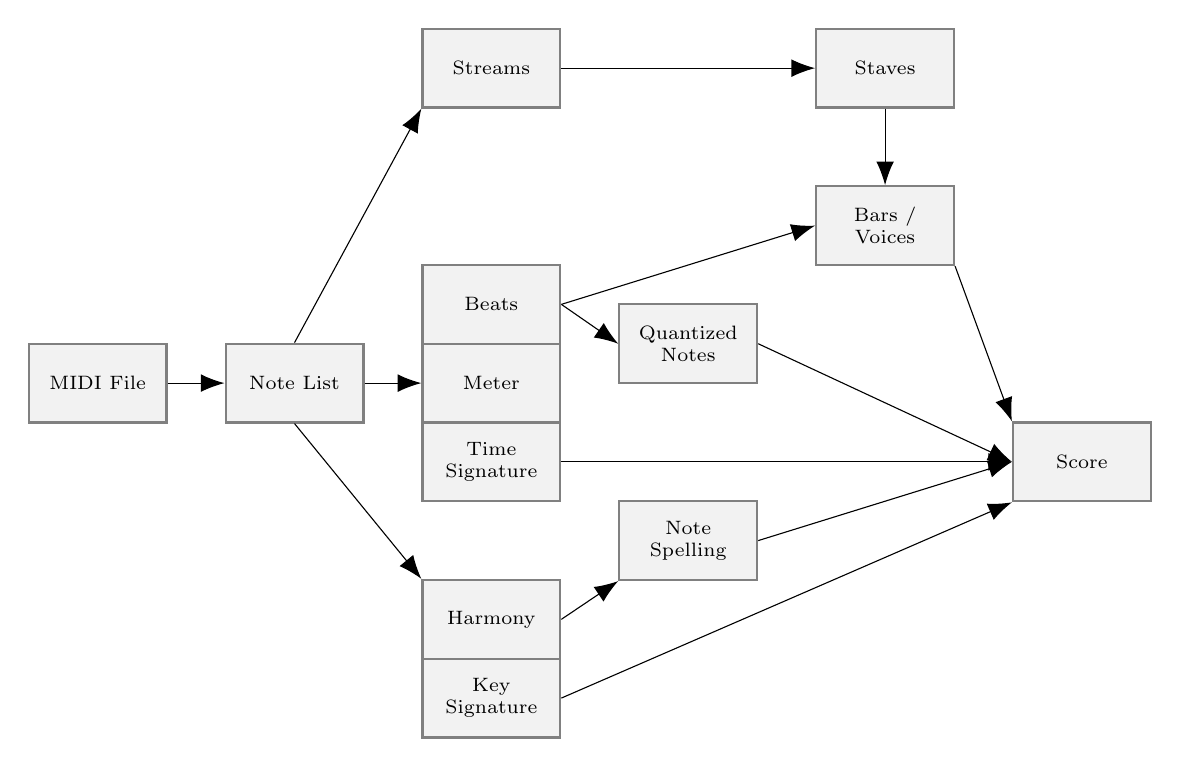
\begin{tikzpicture}
    \tikzset{font=\scriptsize}
    \tikzset{layer/.style={fill=gray!10, draw=gray, thick, text centered, align=center, minimum width=1.75cm, minimum height=1.0cm}}

    \tikzset{arrowstyle/.style={-{Latex[length=3mm]}}}
    \draw (-7.5, 0) node[layer] (midi_file) {MIDI File};
    \draw (-5.0, 0) node[layer] (note_list) {Note List};
    \draw (-2.5, 4.0) node[layer] (streams) {Streams};
    \draw (-2.5, 1.0) node[layer] (beats) {Beats};
    \draw (-2.5, 0) node[layer] (meter) {Meter};
    \draw (-2.5, -1.0) node[layer] (time_signature) {Time \\ Signature};
    \draw (-2.5, -3.0) node[layer] (harmony) {Harmony};
    \draw (-2.5, -4.0) node[layer] (key_signature) {Key \\ Signature};
    \draw (0, 0.5) node[layer] (quantized_notes) {Quantized \\ Notes};
    \draw (0, -2.0) node[layer] (note_spelling) {Note \\ Spelling};
    \draw (2.5, 4.0) node[layer] (staves) {Staves};
    \draw (2.5, 2.0) node[layer] (bars_voices) {Bars / \\ Voices};
    \draw (5.0, -1.0) node[layer] (score) {Score};

    \draw[arrowstyle] (midi_file.east) -- (note_list.west);
    \draw[arrowstyle] (note_list.north) -- (streams.south west);
    \draw[arrowstyle] (note_list.east) -- (meter.west);
    \draw[arrowstyle] (note_list.south) -- (harmony.north west);
    \draw[arrowstyle] (streams.east) -- (staves.west);
    \draw[arrowstyle] (staves.south) -- (bars_voices.north);
    \draw[arrowstyle] (beats.east) -- (bars_voices.west);
    \draw[arrowstyle] (beats.east) -- (quantized_notes.west);
    \draw[arrowstyle] (harmony.east) -- (note_spelling.south west);
    \draw[arrowstyle] (key_signature.east) -- (score.south west);
    \draw[arrowstyle] (note_spelling.east) -- (score.west);
    \draw[arrowstyle] (quantized_notes.east) -- (score.west);
    \draw[arrowstyle] (time_signature.east) -- (score.west);
    \draw[arrowstyle] (bars_voices.south east) -- (score.north west);
\end{tikzpicture}}
\caption{Performance MIDI to score system proposed by Cogliati et al. \cite{Cogliati2016}.}
\end{figure}
\end{frame}

\section{Performance MIDI to Score Conversion}

\begin{frame}
To convert a performance MIDI (a raw stream of notes) to a score, one needs to: \pause\begin{itemize}
	\item Quantize notes: \begin{itemize}
		\item Impose a beat grid.\pause
		\item Align musical onsets to the grid.\pause
		\item Interpret music durations in terms of note values.\pause
	\end{itemize}
	\item Assign time signatures.\pause
	\item Assign key signatures.\pause
	\item Separate left and right hand notes.
\end{itemize}
\end{frame}

\begin{frame}
\begin{figure}[ht!]
\centering
\scalebox{0.7}{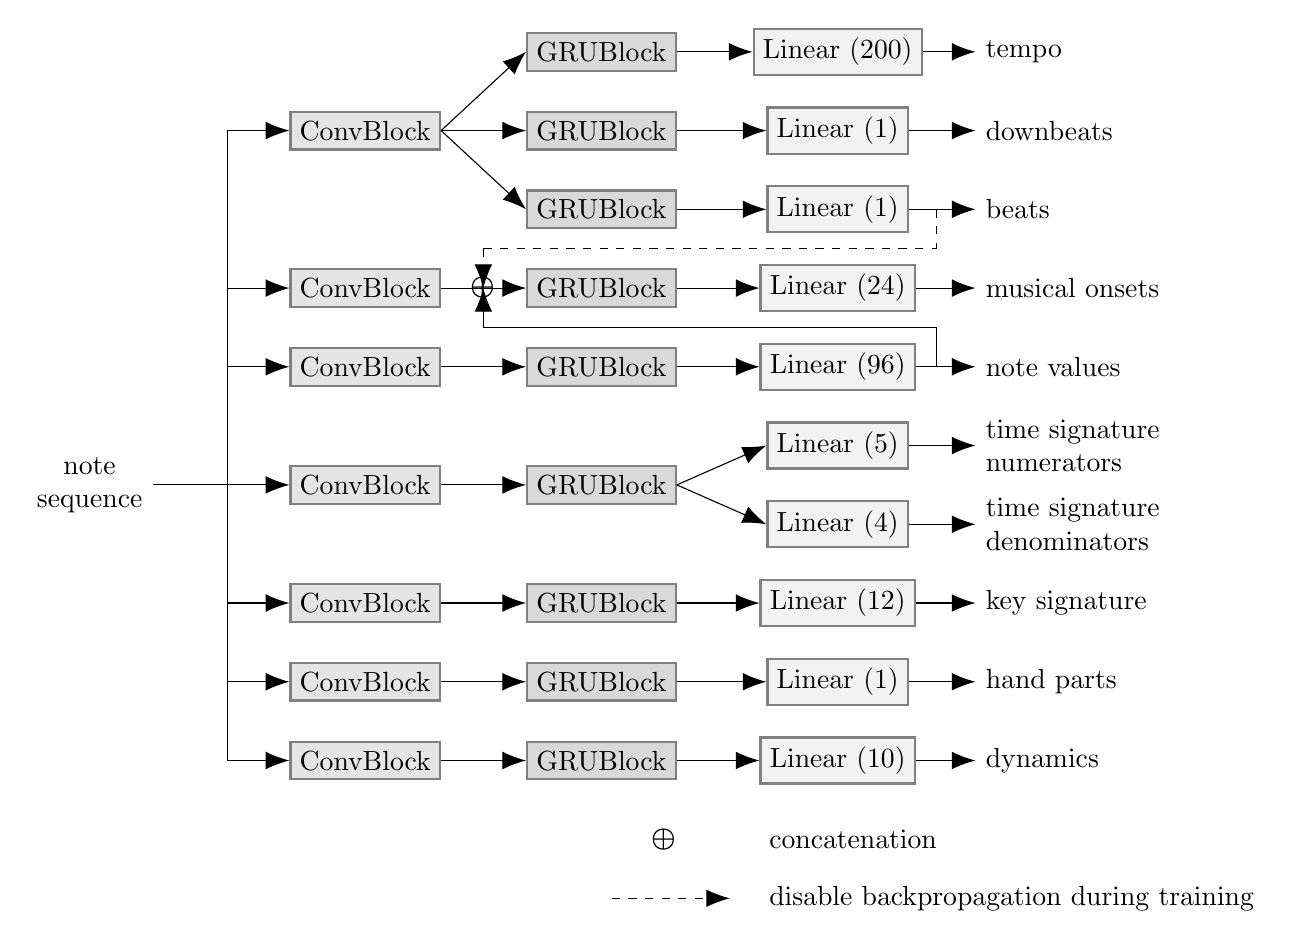
\begin{tikzpicture}
    \tikzset{sequence/.style={thick, text centered, align=center}}
    \tikzset{convblock/.style={fill=gray!20, draw=gray, thick, text centered}}
    \tikzset{grublock/.style={fill=gray!30, draw=gray, thick, text centered}}
    \tikzset{linear/.style={fill=gray!10, draw=gray, thick, text centered}}
    \tikzset{output/.style={thick, anchor=west, align=left}}
    \tikzset{arrowstyle/.style={-{Latex[length=3mm]}}}
    \draw (-3.5, 0.5) node[sequence] (sequence) {note\\ sequence};

    \draw (-1.75, 5) node (joint1) {};
    \draw (-1.75, 3) node (joint2) {};
    \draw (-1.75, 2) node (joint3) {};
    \draw (-1.75, 0.5) node (joint4) {};
    \draw (-1.75, -1) node (joint5) {};
    \draw (-1.75, -2) node (joint6) {};
    \draw (-1.75, -3) node (joint7) {};

    \draw (1.5, 3) node (concatenation) {$\boldsymbol{\oplus}$};
    \draw (1.5, 3.5) node (concatleftjoint1) {};
    \draw (1.5, 2.5) node (concatleftjoint2) {};
    \draw (7.25, 3.5) node (concatrightjoint1) {};
    \draw (7.25, 2.5) node (concatrightjoint2) {};
    \draw (7.25, 2) node (concatstart1) {};
    \draw (7.25, 4) node (concatstart2) {};

    \draw (0, 5) node[convblock] (convblock1) {ConvBlock};
    \draw (0, 3) node[convblock] (convblock2) {ConvBlock};
    \draw (0, 2) node[convblock] (convblock3) {ConvBlock};
    \draw (0, 0.5) node[convblock] (convblock4) {ConvBlock};
    \draw (0, -1) node[convblock] (convblock5) {ConvBlock};
    \draw (0, -2) node[convblock] (convblock6) {ConvBlock};
    \draw (0, -3) node[convblock] (convblock7) {ConvBlock};

    \draw (3, 6) node[grublock] (grublock1) {GRUBlock};
    \draw (3, 5) node[grublock] (grublock2) {GRUBlock};
    \draw (3, 4) node[grublock] (grublock3) {GRUBlock};
    \draw (3, 3) node[grublock] (grublock4) {GRUBlock};
    \draw (3, 2) node[grublock] (grublock5) {GRUBlock};
    \draw (3, 0.5) node[grublock] (grublock6) {GRUBlock};
    \draw (3, -1) node[grublock] (grublock7) {GRUBlock};
    \draw (3, -2) node[grublock] (grublock8) {GRUBlock};
    \draw (3, -3) node[grublock] (grublock9) {GRUBlock};

    \draw (6, 6) node[linear] (linear1) {Linear (200)};
    \draw (6, 5) node[linear] (linear2) {Linear (1)};
    \draw (6, 4) node[linear] (linear3) {Linear (1)};
    \draw (6, 3) node[linear] (linear4) {Linear (24)};
    \draw (6, 2) node[linear] (linear5) {Linear (96)};
    \draw (6, 1) node[linear] (linear6) {Linear (5)};
    \draw (6, 0) node[linear] (linear7) {Linear (4)};
    \draw (6, -1) node[linear] (linear8) {Linear (12)};
    \draw (6, -2) node[linear] (linear9) {Linear (1)};
    \draw (6, -3) node[linear] (linear10) {Linear (10)};

    \draw (7.75, 6) node[output] (output1) {tempo};
    \draw (7.75, 5) node[output] (output2) {downbeats};
    \draw (7.75, 4) node[output] (output3) {beats};
    \draw (7.75, 3) node[output] (output4) {musical onsets};
    \draw (7.75, 2) node[output] (output5) {note values};
    \draw (7.75, 1) node[output] (output6) {time signature\\  numerators};
    \draw (7.75, 0) node[output] (output7) {time signature\\  denominators};
    \draw (7.75, -1) node[output] (output8) {key signature};
    \draw (7.75, -2) node[output] (output9) {hand parts};
    \draw (7.75, -3) node[output] (output10) {dynamics};

    \draw (sequence) to (joint4.center);
    \draw (joint1.center) to (joint7.center);
    \draw[arrowstyle] (joint1.center) to (convblock1);
    \draw[arrowstyle] (joint2.center) to (convblock2);
    \draw[arrowstyle] (joint3.center) to (convblock3);
    \draw[arrowstyle] (joint4.center) to (convblock4);
    \draw[arrowstyle] (joint5.center) to (convblock5);
    \draw[arrowstyle] (joint6.center) to (convblock6);
    \draw[arrowstyle] (joint7.center) to (convblock7);

    \draw[arrowstyle] (convblock1.east) to (grublock1.west);
    \draw[arrowstyle] (convblock1.east) to (grublock2.west);
    \draw[arrowstyle] (convblock1.east) to (grublock3.west);
    \draw[arrowstyle] (convblock2.east) to (grublock4.west);
    \draw[arrowstyle] (convblock3.east) to (grublock5.west);
    \draw[arrowstyle] (convblock4.east) to (grublock6.west);
    \draw[arrowstyle] (convblock5.east) to (grublock7.west);
    \draw[arrowstyle] (convblock6.east) to (grublock8.west);
    \draw[arrowstyle] (convblock7.east) to (grublock9.west);

    \draw[arrowstyle] (grublock1.east) to (linear1.west);
    \draw[arrowstyle] (grublock2.east) to (linear2.west);
    \draw[arrowstyle] (grublock3.east) to (linear3.west);
    \draw[arrowstyle] (grublock4.east) to (linear4.west);
    \draw[arrowstyle] (grublock5.east) to (linear5.west);
    \draw[arrowstyle] (grublock6.east) to (linear6.west);
    \draw[arrowstyle] (grublock6.east) to (linear7.west);
    \draw[arrowstyle] (grublock7.east) to (linear8.west);
    \draw[arrowstyle] (grublock8.east) to (linear9.west);
    \draw[arrowstyle] (grublock9.east) to (linear10.west);

    \draw[arrowstyle] (linear1.east) to (output1.west);
    \draw[arrowstyle] (linear2.east) to (output2.west);
    \draw[arrowstyle] (linear3.east) to (output3.west);
    \draw[arrowstyle] (linear4.east) to (output4.west);
    \draw[arrowstyle] (linear5.east) to (output5.west);
    \draw[arrowstyle] (linear6.east) to (output6.west);
    \draw[arrowstyle] (linear7.east) to (output7.west);
    \draw[arrowstyle] (linear8.east) to (output8.west);
    \draw[arrowstyle] (linear9.east) to (output9.west);
    \draw[arrowstyle] (linear10.east) to (output10.west);

    \draw[arrowstyle, dashed] (concatleftjoint1.center) to (concatenation.center);
    \draw[arrowstyle] (concatleftjoint2.center) to (concatenation.center);
    \draw[dashed] (concatleftjoint1.center) to (concatrightjoint1.center);
    \draw (concatleftjoint2.center) to (concatrightjoint2.center);
    \draw (concatstart1.center) to (concatrightjoint2.center);
    \draw[dashed] (concatstart2.center) to (concatrightjoint1.center);

    \draw (3.5, -4) node[output] (legendsymbol1) {$\boldsymbol{\oplus}$};
    \draw (3, -4.75) node[output] (legendsymbolstart) {};
    \draw (4.5, -4.75) node[output] (legendsymbolend) {};
    \draw (5, -4) node[output] (legend1) {concatenation};
    \draw (5, -4.75) node[output] (legend2) {disable backpropagation during training};
    \draw[arrowstyle, dashed] (legendsymbolstart.center) to (legendsymbolend.center);
\end{tikzpicture}
}
\caption{The main model's architecture. The dynamics submodule is a novel part.}
\end{figure}
\end{frame}

\section{Analysis}

\begin{frame}
We reproduced the results using the same setup as the authors:
\begin{table}[ht!]
\centering
\begin{tabular}{c|cccccc}
    \textbf{Model} & $F_{\textrm{p}}$ & $F_{\textrm{vs}}$ & $F_{\textrm{ma}}$ & $F_{\textrm{nv}}$ & $F_{\textrm{ha}}$ & $F$ \\\hline
    Original       & $\mathbf{0.998}$ & $\mathbf{0.870}$  & $\mathbf{0.617}$  & $0.999$           & $0.911$           & $0.879$          \\
    Reproduced     & $0.986$          & $0.826$           & $0.598$           & $\mathbf{1.000}$  & $\mathbf{1.000}$  & $\mathbf{0.882}$ \\
\end{tabular}

\caption[MV2H metric evaluation on the test set.]{MV2H metric evaluation on the test set, with results compared to the original model evaluation.}
\end{table}
\end{frame}

\subsection{Case Studies}

\begin{frame}
\begin{figure}[ht!]
\centering
\begin{tabular}{c}a)
\includesvg[width=0.95\textwidth]{images/albeniz_gen.svg} \\ b)
\includesvg[width=0.95\textwidth]{images/albeniz_output_gen.svg}
\end{tabular}
\caption[\emph{Sevilla} by Isaac Albéniz.]{\emph{Sevilla} by Isaac Albéniz: a) the piece with a distinguished pickup measure (first three notes for each hand), b) the model transcription. Since the model assumed the time signature of $\lilyTimeSignature{3}{4}$, the resulting content is shifted by the half of a measure. Other musical elements have been correctly assigned.}
\label{albeniz}
\end{figure}
\end{frame}

\begin{frame}
\begin{figure}[ht!]
\centering \begin{tabular}{c}a) \includesvg[width=0.95\textwidth]{images/claire_de_lune_gen.svg} \\ b) \includesvg[width=0.95\textwidth]{images/claire_de_lune_output_gen.svg} \end{tabular} \caption[Claude Debussy's \emph{Clair de Lune}.]{The beginning of Claude Debussy's \emph{Clair de Lune}: a) the original score from the MAPS test dataset, b) the model transcription. The model misaligned the metric structure by mixing quarter notes with triplets, disrupting the inner relationships between notes within a measure. Some right-hand notes (e.g., C in the second measure) are misattributed. The key signature was assigned correctly.}
\label{claire_de_lune}
\end{figure}
\end{frame}

\subsection{\emph{Ceteris Paribus} Analysis}

\begin{frame}
We conducted a \emph{ceteris paribus} type of analysis by augmenting original note sequence tensors to test if the model satisfies some natural requirements:\pause \begin{itemize}
	\item Note velocity should not influence time signature or hand part assignment.\pause
	\item Note pitch should be irrelevant to time signature prediction.\pause
	\item Note pitch is essential for determining key signature and hand part assignment, while other features should have minimal impact on these aspects.\pause
	\item Note duration should not affect key signature assignment.
\end{itemize}
\end{frame}

\begin{frame}
For a sample $M = 50$ musical pieces from the dataset, we introduced the following transformations:\pause \begin{itemize}
	\item Adding noise to the velocity of different standard deviations $\sigma_v$.\pause
	\item Scaling note lengths by a factor.\pause
	\item Changing pitch with standard deviations $\sigma_p$.
\end{itemize}
\end{frame}

\begin{frame}
\begin{figure}[ht!]
\centering
\includesvg[width=1.0\textwidth]{images/ceteris_paribus_results_h.svg}
\caption{Results of the \emph{ceteris paribus} experiment for the hand part model $f_H$. The model is robust to note duration changes while it is susceptible to velocity manipulation.}
\end{figure}
\end{frame}

\begin{frame}
\begin{figure}[ht!]
\centering
\includesvg[width=1.0\textwidth]{images/ceteris_paribus_results_k.svg}
\caption{Results of the \emph{ceteris paribus} experiment for the key signature model $f_K$. The model is robust to all perturbations.}
\end{figure}
\end{frame}

\begin{frame}
\begin{figure}[ht!]
\centering
\includesvg[width=1.0\textwidth]{images/ceteris_paribus_results_t.svg}
\caption{Results of the \emph{ceteris paribus} experiment for the time signature model $f_T$. The model is sensitive to note duration changes, which is expected to some extent, and relatively robust to other transformations.}
\end{figure}
\end{frame}

\subsection{Local Feature Importance}

\begin{frame}
We developed a custom XAI methods to better understand the model's decisions. In particular, we wanted to know the influence of individual notes on model output.\pause

For instance, we used a LIME-like approach to assess how the model velocity affects the hand part assignment on the note level.
\end{frame}

\begin{frame}
\begin{figure}[ht!] \centering \includesvg[width=0.85\textwidth]{images/lime_hand_part.svg} \caption[Velocity influence on hand part assignment.]{Velocity influence on hand part assignment. The G2 note (thick outline) is influenced by the velocity of neighboring notes. Negative influence is represented by the diagonal pattern. Increasing the velocity of the low note causes misalignment of G3 and B3 notes to the left hand, while reducing the G2 velocity shifts it to the right hand. This behavior is undesirable.} \label{hand_part_misalignment} \end{figure}
\end{frame}

\begin{frame}
For key signature assignment, we developed a method for measuring individual note influence on the assignment.\pause

To measure if a particular note voted for or against the current note, we calculated the difference between model's decision on the original sequence and model's output on a sequence with the note being removed. 
\end{frame}

\section{Experiments}

\begin{frame}
We conducted several experiments:\pause
\begin{itemize}
	\item Perform ablation studies based on the XAI observations.\pause
	\item Explore the Transformed-based networks.\pause
	\item Test smaller, data-efficient networks to optimize the current architecture.\pause
	\item Extend the model by the dynamics model. \end{itemize}
\end{frame}

\subsection{Ablation Studies}

\begin{frame}Based on previous observations, we extended the original research by conducting several ablation studies:\pause \begin{itemize}
	\item The \textbf{hand part} model was trained only on note pitches and onsets.\pause
	\item The \textbf{key signature} model was trained only on note pitches and onsets.\pause
	\item The \textbf{time signature} model was trained using only note onsets.\pause
\end{itemize}

We proved that excluding velocity from hand part and time signature models doesn't hurt the overall performance of the model.  The restricted time signature model was superior to the original model.
\end{frame}

\subsection{Transformers}

\begin{frame}
\begin{figure}[ht!]
\centering
\resizebox{!}{0.8\textheight}{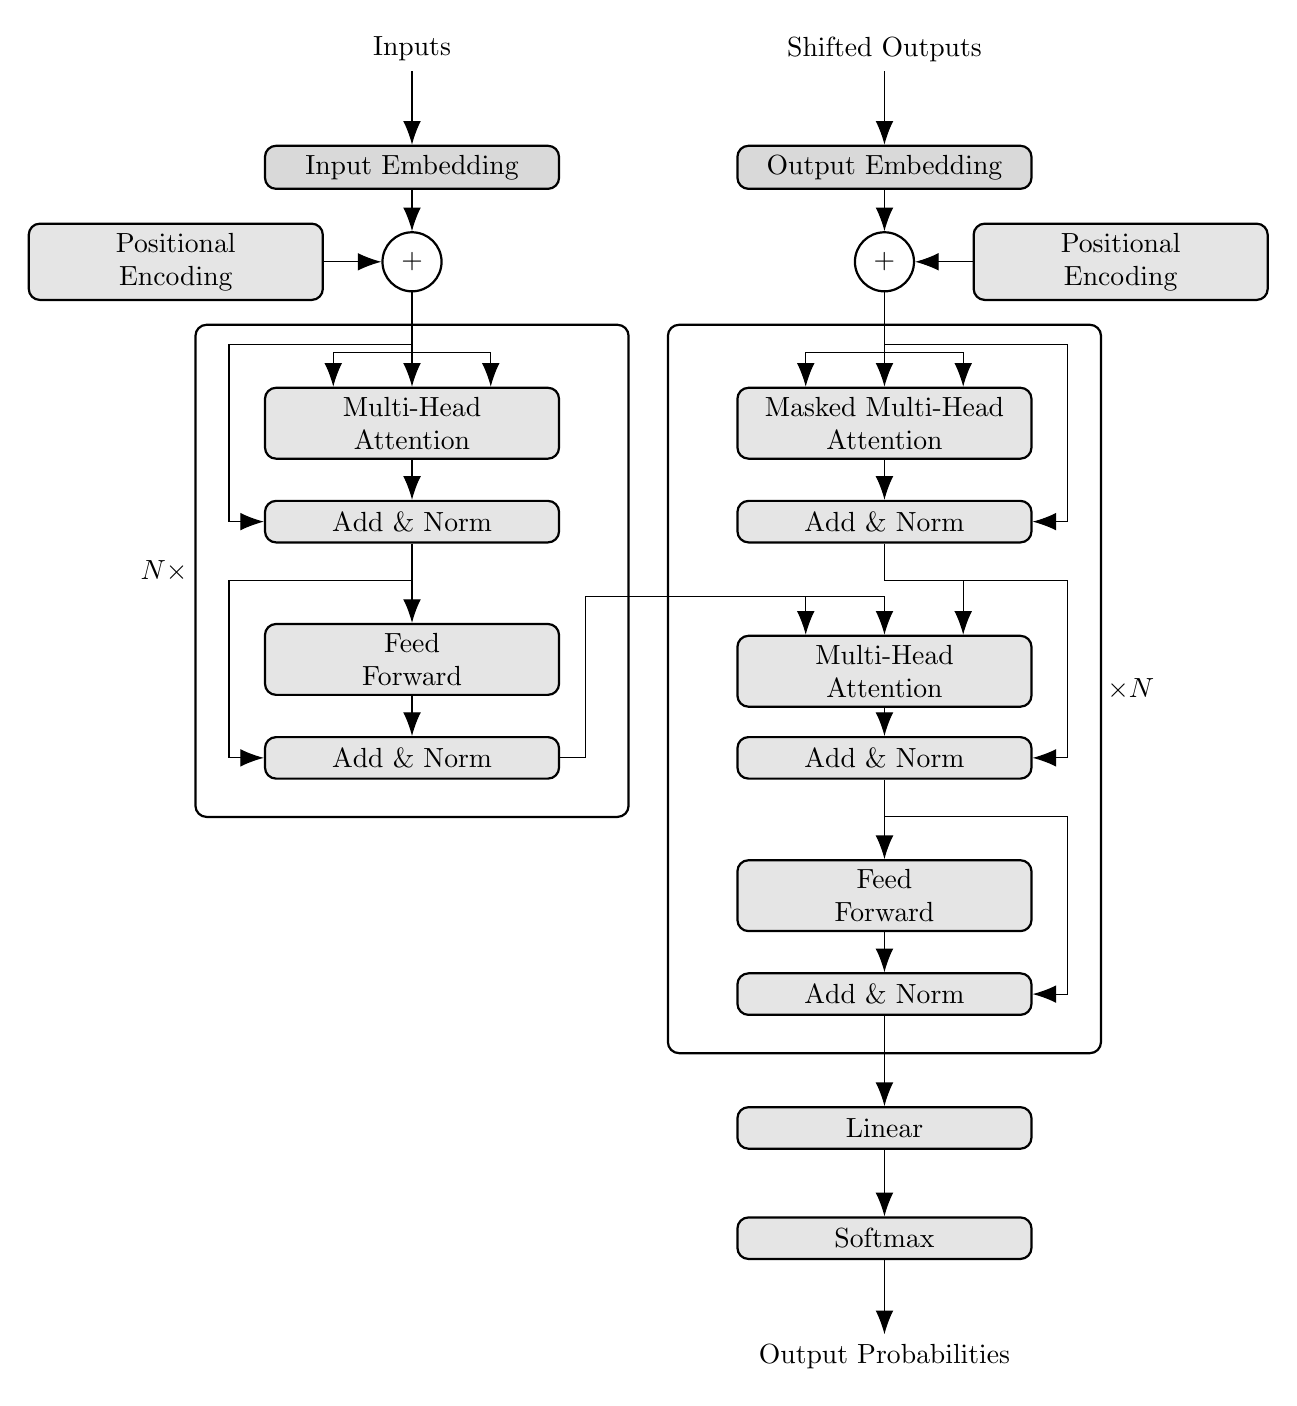
\begin{tikzpicture}
    \tikzset{block/.style={fill=gray!20, text width=3.5cm, draw=black, thick, text centered, align=center, rounded corners, minimum height=1.5em, minimum width=3.5cm}}
    \tikzset{input/.style={fill=gray!30, text width=3.5cm, draw=black, thick, text centered, rounded corners, minimum height=1.5em, minimum width=3.5cm}}
    \tikzset{operation/.style={draw, circle, thick, minimum size=0.75cm}}
    \tikzset{arrowstyle/.style={-{Latex[length=3mm]}}}

    \node (inputs) at (0, 1.5) {Inputs};
    \node (outputs) at (6, 1.5) {Shifted Outputs};

    \node[input] (input_embed) at (0, 0) {Input Embedding};
    \node[block] (pos_encoding) at (-3, -1.2) {Positional \\ Encoding};
    \node[operation] (add1) at (0, -1.2) {$+$};

    \node[block] (multihead1) at (0, -3.25) {Multi-Head \\ Attention};
    \node[block] (add_norm1) at (0, -4.5) {Add \& Norm};
    \node[block] (ffn1) at (0, -6.25) {Feed \\ Forward};
    \node[block] (add_norm2) at (0, -7.5) {Add \& Norm};

    \draw[rounded corners, thick] (-2.75, -2) rectangle (2.75, -8.25) node[pos=0.5, xshift=-3.1cm] {$N \times \;$};

    \node[input] (output_embed) at (6, 0) {Output Embedding};
    \node[block] (pos_encoding_dec) at (9, -1.2) {Positional \\ Encoding};
    \node[operation] (add2) at (6, -1.2) {$+$};

    \node[block] (masked_mha) at (6, -3.25) {Masked Multi-Head \\ Attention};
    \node[block] (add_norm_dec1) at (6, -4.5) {Add \& Norm};
    \node[block] (mha_dec) at (6, -6.40) {Multi-Head \\ Attention};
    \node[block] (add_norm_dec2) at (6, -7.50) {Add \& Norm};
    \node[block] (ffn2) at (6, -9.25) {Feed \\ Forward};
    \node[block] (add_norm_dec3) at (6, -10.50) {Add \& Norm};

    \draw[rounded corners, thick] (3.25, -2) rectangle (8.75, -11.25) node[pos=0.5, xshift=3.1cm] {$\, \times N$};

    \node[block] (linear) at (6, -12.2) {Linear};
    \node[block] (softmax) at (6, -13.6) {Softmax};
    \node (output_probs) at (6, -15.1) {Output Probabilities};

    \draw[arrowstyle] (inputs.south) -- (input_embed.north);
    \draw[arrowstyle] (input_embed.south) -- (add1.north);
    \draw[arrowstyle] (pos_encoding.east) -- (add1.west);
    \draw[arrowstyle] (add1) -- (multihead1);
    \draw[arrowstyle] (multihead1) -- (add_norm1);
    \draw[arrowstyle] (add_norm1) -- (ffn1);
    \draw[arrowstyle] (ffn1) -- (add_norm2);

    \draw[arrowstyle] (outputs.south) -- (output_embed.north);
    \draw[arrowstyle] (output_embed.south) -- (add2.north);
    \draw[arrowstyle] (pos_encoding_dec.west) -- (add2.east);
    \draw[arrowstyle] (add2) -- (masked_mha);
    \draw[arrowstyle] (masked_mha) -- (add_norm_dec1);
    \draw[arrowstyle] (mha_dec) -- (add_norm_dec2);
    \draw[arrowstyle] (add_norm_dec2) -- (ffn2);
    \draw[arrowstyle] (ffn2) -- (add_norm_dec3);
    \draw[arrowstyle] (add_norm_dec3) -- (linear);
    \draw[arrowstyle] (linear) -- (softmax);
    \draw[arrowstyle] (softmax) -- (output_probs);

    \draw[arrowstyle] (add_norm2.east) -| ++(0.325, 0) |- ++(0, 2.05) -| ($(mha_dec.north) - (1.0, 0.0)$);
    \draw[arrowstyle] (add_norm2.east) -| ++(0.325, 0) |- ++(0, 2.05) -| (mha_dec.north);

    \draw[arrowstyle] (0, -2.25) -| ++(-2.325,0) |- (add_norm1.west);
    \draw[arrowstyle] (0, -5.25) -| ++(-2.325,0) |- (add_norm2.west);

    \draw[arrowstyle] (0, -2.35) -| ++(-1.0,0) -- ($(multihead1.north) - (1.0, 0.0)$);
    \draw[arrowstyle] (0, -2.35) -| ++(1.0,0) -- ($(multihead1.north) + (1.0, 0.0)$);

    \draw[arrowstyle] (6, -2.35) -| ++(-1.0,0) -- ($(masked_mha.north) - (1.0, 0.0)$);
    \draw[arrowstyle] (6, -2.35) -| ++(1.0,0) -- ($(masked_mha.north) + (1.0, 0.0)$);

    \draw[arrowstyle] (add_norm_dec1) -- (6, -5.25) -| ++(1.0,0) -- ($(mha_dec.north) + (1.0, 0.0)$);

    \draw[arrowstyle] (6, -2.25) -| ++(2.325,0) |- (add_norm_dec1.east);
    \draw[arrowstyle] (6, -5.25) -| ++(2.325,0) |- (add_norm_dec2.east);
    \draw[arrowstyle] (6, -8.25) -| ++(2.325,0) |- (add_norm_dec3.east);

\end{tikzpicture}}
\caption[The Transformer architecture.]{The Transformer architecture \cite{Vaswani2017}.}
\end{figure}
\end{frame}

\begin{frame}
\begin{figure}[ht!]
\centering
\resizebox{\textwidth}{!}{
\begin{tabular}{cc}a)
\scalebox{0.8}{
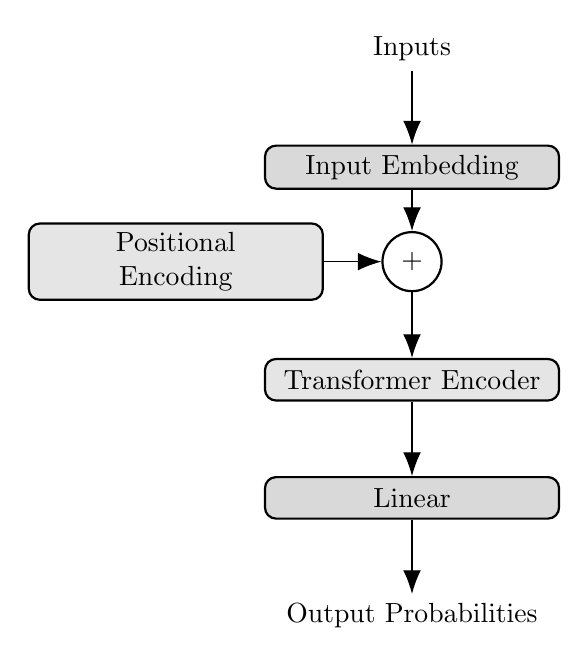
\begin{tikzpicture}
    \tikzset{block/.style={fill=gray!20, text width=3.5cm, draw=black, thick, text centered, align=center, rounded corners, minimum height=1.5em, minimum width=3.5cm}}
    \tikzset{input/.style={fill=gray!30, text width=3.5cm, draw=black, thick, text centered, rounded corners, minimum height=1.5em, minimum width=3.5cm}}
    \tikzset{operation/.style={draw, circle, thick, minimum size=0.75cm}}
    \tikzset{arrowstyle/.style={-{Latex[length=3mm]}}}

    \node (inputs) at (0, 1.5) {Inputs};
    \node[input] (input_embed) at (0, 0) {Input Embedding};
    \node[block] (pos_encoding) at (-3, -1.2) {Positional \\ Encoding};
    \node[operation] (add) at (0, -1.2) {$+$};
    \node[block] (transformer) at (0, -2.7) {Transformer Encoder};
    \node[input] (linear) at (0, -4.2) {Linear};
    \node (output) at (0, -5.7) {Output Probabilities};

    \draw[arrowstyle] (inputs.south) -- (input_embed.north);
    \draw[arrowstyle] (input_embed.south) -- (add.north);
    \draw[arrowstyle] (pos_encoding.east) -- (add.west);
    \draw[arrowstyle] (add) -- (transformer);
    \draw[arrowstyle] (transformer) -- (linear);
    \draw[arrowstyle] (linear) -- (output);

\end{tikzpicture}
} & b)
\scalebox{0.8}{
    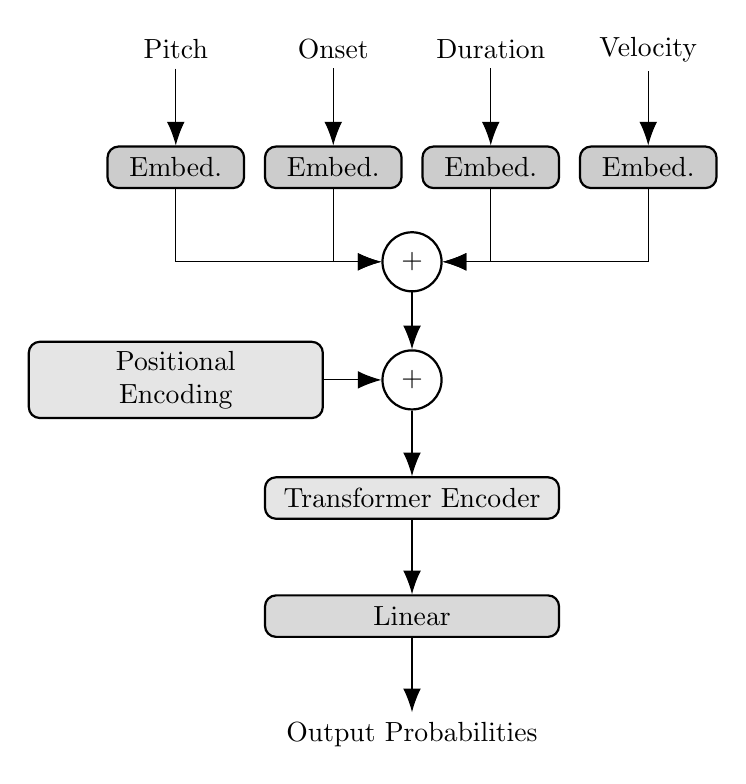
\begin{tikzpicture}
    \tikzset{block/.style={fill=gray!20, text width=3.5cm, draw=black, thick, text centered, align=center, rounded corners, minimum height=1.5em, minimum width=3.5cm}}
    \tikzset{input/.style={fill=gray!30, text width=3.5cm, draw=black, thick, text centered, rounded corners, minimum height=1.5em, minimum width=3.5cm}}
    \tikzset{embedding/.style={fill=gray!40, text width=1.5cm, draw=black, thick, text centered, rounded corners, minimum height=1.5em, minimum width=1.5cm}}
    \tikzset{operation/.style={draw, circle, thick, minimum size=0.75cm}}
    \tikzset{arrowstyle/.style={-{Latex[length=3mm]}}}

    \node (pitch) at (-3.0, 1.5) {Pitch};
    \node (onset) at (-1.0, 1.5) {Onset};
    \node (duration) at (1.0, 1.5) {Duration};
    \node (velocity) at (3.0, 1.5) {Velocity};
    \node[embedding] (pitch_embed) at (-3.0, 0) {Embed.};
    \node[embedding] (onset_embed) at (-1.0, 0) {Embed.};
    \node[embedding] (duration_embed) at (1.0, 0) {Embed.};
    \node[embedding] (velocity_embed) at (3.0, 0) {Embed.};
    \node[block] (pos_encoding) at (-3, -2.7) {Positional \\ Encoding};
    \node[operation] (add1) at (0, -1.2) {$+$};
    \node[operation] (add2) at (0, -2.7) {$+$};
    \node[block] (transformer) at (0, -4.2) {Transformer Encoder};
    \node[input] (linear) at (0, -5.7) {Linear};
    \node (output) at (0, -7.2) {Output Probabilities};

    \draw[arrowstyle] (pitch.south) -- (pitch_embed.north);
    \draw[arrowstyle] (onset.south) -- (onset_embed.north);
    \draw[arrowstyle] (duration.south) -- (duration_embed.north);
    \draw[arrowstyle] (velocity.south) -- (velocity_embed.north);
    \draw[arrowstyle] (pitch_embed.south) |- (add1.west);
    \draw[arrowstyle] (onset_embed.south) |- (add1.west);
    \draw[arrowstyle] (duration_embed.south) |- (add1.east);
    \draw[arrowstyle] (velocity_embed.south) |- (add1.east);
    \draw[arrowstyle] (pos_encoding.east) -- (add2.west);
    \draw[arrowstyle] (add1) -- (add2);
    \draw[arrowstyle] (add2) -- (transformer);
    \draw[arrowstyle] (transformer) -- (linear);
    \draw[arrowstyle] (linear) -- (output);

\end{tikzpicture}
}
\end{tabular}}
\caption[The Transformer Encoder block.]{The Transformer Encoder block: a) default encoding, b) feature embedding. The $\frown$ symbols stands for concatenation. The second architecture was selected for subsequent experiments. The positional encoding is optional.}
\label{vanilla_transformer_encoder_with_embedding}
\end{figure}
\end{frame}

\begin{frame}
Transformed-based beat model not only didn't outperform the base model, but it was significantly worse. Similarly, but in less extent, for the hand part model.\pause

Key and time signature Transformers were on par with the base model.\pause

In most cases, the sinusoidal positional encoding worsened the results.
\end{frame}

\subsection{Temporal Convolutional Network}

\begin{frame}
\begin{figure}[ht!]
\centering
\resizebox{!}{0.8\textheight}{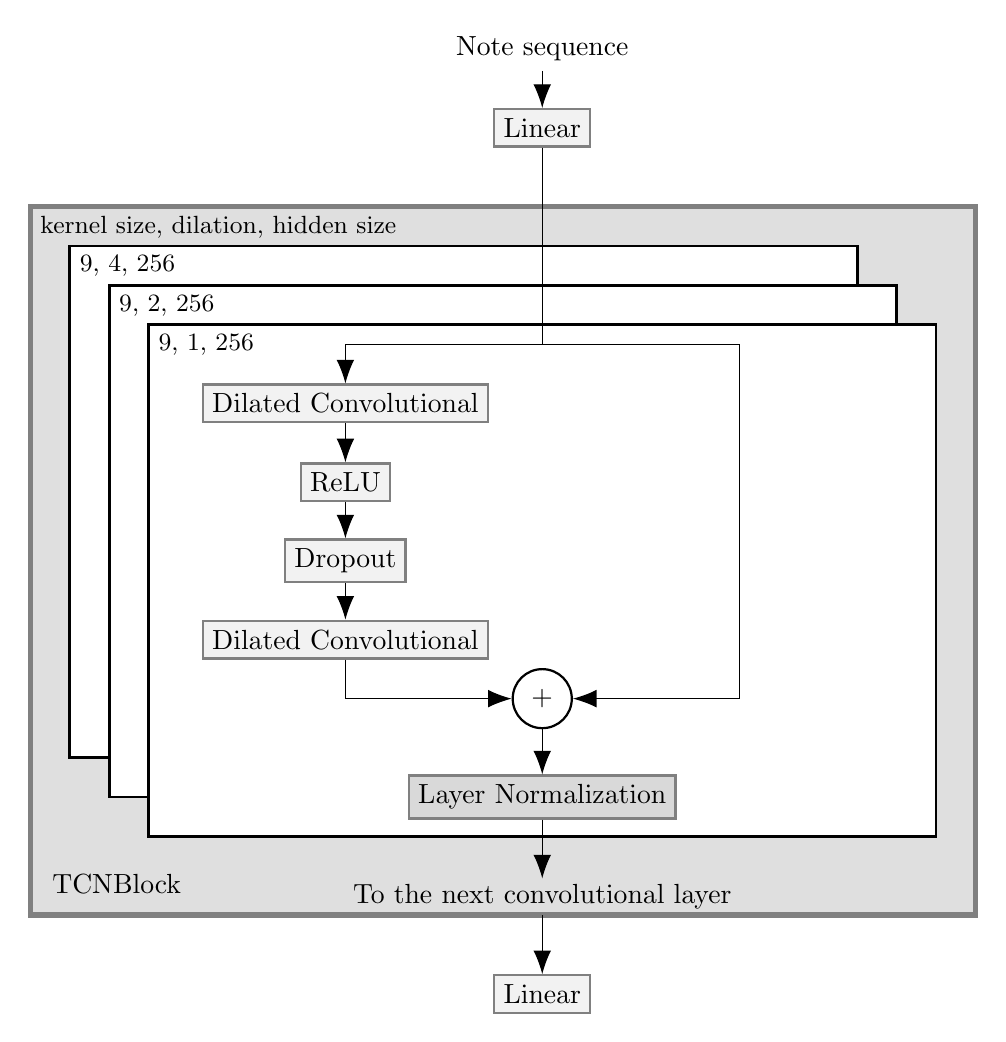
\begin{tikzpicture}
    \tikzset{layer1/.style={fill=gray!10, draw=gray, thick, text centered}}
    \tikzset{layer2/.style={fill=gray!30, draw=gray, thick, text centered}}
    \tikzset{operation/.style={draw, circle, thick, minimum size=0.75cm}}
    \tikzset{arrowstyle/.style={-{Latex[length=3mm]}}}

    \fill[fill=gray!50, fill opacity=0.5, draw=gray, thick, line width=2pt] (0.0, -2.0) rectangle (12.0, 7.0);
    \fill[fill=white!50, fill opacity=1.0, draw=black, thick, line width=1pt] (0.5, 0.0) rectangle (10.5, 6.5);
    \fill[fill=white!50, fill opacity=1.0, draw=black, thick, line width=1pt] (1.0, -0.5) rectangle (11.0, 6.0);
    \fill[fill=white!50, fill opacity=1.0, draw=black, thick, line width=1pt] (1.5, -1.0) rectangle (11.5, 5.5);

    \draw (6.5, 9.00) node (note_sequence) {Note sequence};
    \draw (6.5, 8.00) node[layer1] (embedding) {Linear};
    \draw (4.0, 4.50) node[layer1] (layerA1) {Dilated Convolutional};
    \draw (4.0, 3.50) node[layer1] (layerA2) {ReLU};
    \draw (4.0, 2.50) node[layer1] (layerA3) {Dropout};
    \draw (4.0, 1.50) node[layer1] (layerA4) {Dilated Convolutional};
    \draw (6.5, 0.75) node[operation] (add) {$+$};
    \draw (6.5, -0.50) node[layer2] (layerA5) {Layer Normalization};
    \draw[anchor=south, inner sep=2pt] (6.5, -2.0) node (outputA) {To the next convolutional layer};

    \draw (6.5, -3.00) node[layer1] (output) {Linear};

    \node[anchor=south west, inner sep=2pt] at (0.2, -1.8) {TCNBlock};

    \node[anchor=north west, inner sep=2pt] at (1.55, 5.45) {\small{9, 1, 256}};
    \node[anchor=north west, inner sep=2pt] at (1.05, 5.95) {\small{9, 2, 256}};
    \node[anchor=north west, inner sep=2pt] at (0.55, 6.45) {\small{9, 4, 256}};
    \node[anchor=north west, inner sep=2pt] at (0.05, 6.95) {\small{kernel size, dilation, hidden size}};

    \draw[arrowstyle] (note_sequence.south) to (embedding.north);
    \draw[arrowstyle] (embedding.south) -| ++(0.0, -2.5) -| (layerA1.north);
    \draw[arrowstyle] (embedding.south) -| ++(0.0, -2.5) -| ++(2.5, 0.0) |- (add.east);
    \draw[arrowstyle] (layerA1.south) to (layerA2.north);
    \draw[arrowstyle] (layerA2.south) to (layerA3.north);
    \draw[arrowstyle] (layerA3.south) to (layerA4.north);
    \draw[arrowstyle] (layerA4.south) |- (add.west);
    \draw[arrowstyle] (add.south) to (layerA5.north);
    \draw[arrowstyle] (layerA5.south) to (outputA.north);
    \draw[arrowstyle] (outputA.south) to (output.north);
\end{tikzpicture}
}
\caption[The Temporal Convolutional Block.]{The Temporal Convolutional Block.}
\label{temporal_convolutional_network}
\end{figure}
\end{frame}

\begin{frame}
The TCN networks were on par for each submodel except the key signature model. The TCN time signature model outperformed the base model.
\end{frame}

\subsection{Dynamics Module}

\begin{frame}
We extended the model by a \textbf{dynamics submodule}.\pause

Unfortunately, at the moment the dataset does not contain direct information on dynamics.\pause

The indirect dynamics markings were available only for the ASAP subset.\pause

Only about $60\%$ of all dynamics markings have been extracted from the MusicXML source to annotations.\pause

The model had $F$ score of $0.5$.
\end{frame}

\begin{frame}[allowframebreaks]
\bibliography{bibliography/bibliography}
\end{frame}

\end{document}
